\documentclass[11pt,letterpaper]{article}
\usepackage[margin=2cm]{geometry}
\usepackage{amsmath,amssymb,graphicx,xcolor,booktabs,tabularx,enumitem,titlesec,fancyhdr,array,longtable}
\usepackage{tikz}
\usetikzlibrary{arrows.meta,positioning,shapes.geometric,calc}
\usepackage[hidelinks]{hyperref}
\usepackage{helvet}\renewcommand{\familydefault}{\sfdefault}
\usepackage{microtype}
\titleformat{\section}{\Large\bfseries\color{blue!50!black}}{\thesection}{0.6em}{}
\titleformat{\subsection}{\large\bfseries}{\thesubsection}{0.6em}{}
\setlength{\headheight}{14pt}
\pagestyle{fancy}\fancyhf{}\lhead{sPHENIX Self-Paced Course}\rhead{Module 10: Case studies and ML}\cfoot{\thepage}
\newcommand{\conceptbox}[2]{\par\medskip\noindent\fcolorbox{blue!50!black}{blue!5}{\begin{minipage}{0.96\linewidth}\textbf{#1}\par\smallskip #2\end{minipage}}\par\medskip}
\newcommand{\connectbox}[1]{\par\medskip\noindent\fcolorbox{green!40!black}{green!5}{\begin{minipage}{0.96\linewidth}\textbf{Connect to your analysis}\par\smallskip #1\end{minipage}}\par\medskip}
\newcommand{\pitfallbox}[1]{\par\medskip\noindent\fcolorbox{red!50!black}{red!4}{\begin{minipage}{0.96\linewidth}\textbf{Pitfalls}\par\smallskip #1\end{minipage}}\par\medskip}
\newcommand{\hd}[1]{\par\smallskip\noindent\textbf{\color{blue!50!black}#1.}\ }
\newenvironment{casetab}{\par\smallskip\noindent\small\tabularx{\linewidth}{@{}>{\bfseries}p{2.6cm}X@{}}\toprule}{\bottomrule\endtabularx\par\medskip}
\setlist{itemsep=1pt,topsep=3pt}
\setlength{\emergencystretch}{2em}
\setlength{\parindent}{0pt}\setlength{\parskip}{4pt}
\begin{document}
\begin{center}{\LARGE\bfseries sPHENIX Self-Paced Course --- Module 10}\\[4pt]
{\Large Case studies from the 2026 school and machine learning in sPHENIX}\\[8pt]
Prepared for P.\,D.\ Lewis (Ohio University) \quad November 2026\end{center}

\tableofcontents
\newpage

\section*{How to use this module}
\addcontentsline{toc}{section}{How to use this module}
This module is self-contained. It does not assume that you have seen the slides or recordings of the school. Each case study
explains the physics from first principles, then the method, then what it teaches you. The talks are listed as \emph{sources}, cited
[S\#\#]; all numbers quoted are public design values, textbook or PDG values, or explicitly labelled toy numbers. Results shown at the
school that are internal or preliminary are described only qualitatively.

\hd{Learning objectives} After this module you will be able to:
\begin{itemize}
\item take any sPHENIX analysis apart into question, observable, data, method, key challenge and lessons;
\item explain the physics and method of sixteen student analyses spanning all four topical groups and detector work;
\item recognise the recurring tools (mixing and rotation backgrounds, ABCD purity, tag-and-probe, reference spectra, closure tests);
\item set up a supervised ML classifier or regressor for a physics task, choose its loss, validate it on data and assign systematics;
\item write a two-page capstone proposal tied to your $\pi^0$/$\eta$ cross-section analysis.
\end{itemize}
\hd{Prerequisites} All earlier modules; Module 9 is used most. Basic Python is helpful for the ML part.

\hd{Estimated time} 14 hours (two weeks), plus the capstone proposal.

\hd{Sources (sPHENIX School 2026 flash talks)} [S26] C.-W.\ Shih; [S25] H.-R.\ Jheng; [S34] I.\ Omae; [S37] J.\ Singh;
[S39] L.\ Mwibanda; [S38] K.\ Gable; [S35] R.\ Takaaze; [S40] M.\ I.\ Abdulhamid; [S29] B.\ Sayki; [S32] S.-Y.\ Chen;
[S30] J.\ Hwang; [S31] R.\ Koike; [S41] T.\ Harada; [S27] A.\ Patton; [S28] T.\ Kikuchi; [S42] A.\ M.\ Khan. Supporting talks:
[S05] Bulk TG, [S04] Cold QCD TG, [S17] Photon reconstruction, [S43] Jet analysis. Full titles are in the references.

\hd{Public readings} sPHENIX papers on Au+Au multiplicity (arXiv:2504.02240), transverse energy (arXiv:2504.02242), dijet imbalance
(arXiv:2606.17184) and isolated prompt photons (arXiv:2607.03892).

%======================================================================
\section{How to read an analysis}
\hd{Goal} Learn a fixed template that turns any talk, note or paper into six answers. You will use it for every case study and for your
own capstone.

\begin{enumerate}
\item \textbf{Question.} What physics question is asked? Which theory quantity does the answer constrain?
\item \textbf{Observable.} What is measured, defined precisely enough to compute in a generator?
\item \textbf{Data.} Collision system, run period, trigger, readout mode (triggered or streaming), detectors required, simulation.
\item \textbf{Method.} Reconstruction, signal extraction, background estimation, corrections, normalisation.
\item \textbf{Key challenge.} The one step that limits precision or validity.
\item \textbf{Lesson for you.} What transfers to your $\pi^0$/$\eta$ cross section or $R_{CP}$ work.
\end{enumerate}

\begin{center}
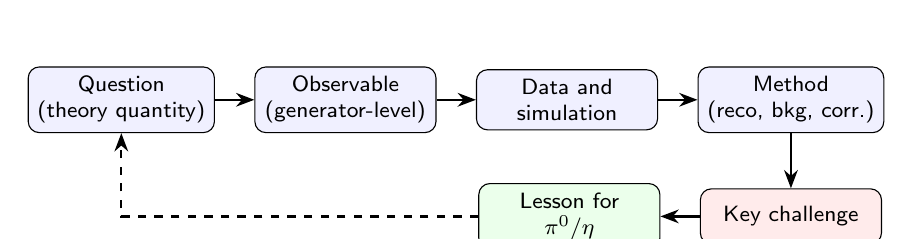
\begin{tikzpicture}[node distance=4mm and 5mm, every node/.style={font=\footnotesize},
 box/.style={draw, rounded corners, fill=blue!6, minimum width=2.3cm, minimum height=7mm, align=center},
 arr/.style={-{Stealth}, thick}]
\node[box] (q) {Question\\(theory quantity)};
\node[box, right=of q] (o) {Observable\\(generator-level)};
\node[box, right=of o] (d) {Data and\\simulation};
\node[box, right=of d] (m) {Method\\(reco, bkg, corr.)};
\node[box, below=7mm of m, fill=red!8] (c) {Key challenge};
\node[box, left=of c, fill=green!8] (l) {Lesson for\\$\pi^0$/$\eta$};
\draw[arr] (q)--(o); \draw[arr] (o)--(d); \draw[arr] (d)--(m); \draw[arr] (m)--(c); \draw[arr] (c)--(l);
\draw[arr, dashed] (l.west) -| (q.south);
\end{tikzpicture}\\[2pt]
{\small Figure 1 (schematic): the six-question template. The dashed arrow: lessons change the questions you ask next.}
\end{center}

Three recurring ideas appear in nearly every case below. Look for them.
\begin{itemize}
\item \textbf{Destroy the signal, keep the detector.} Event mixing, layer rotation and like-sign pairs all estimate combinatorial
background by breaking physical correlations while keeping acceptance.
\item \textbf{Use a reference.} A summed ring spectrum, an average run, a second method, or an independent detector provides the
baseline against which a deviation is measured.
\item \textbf{Close the loop in simulation.} Every correction is applied to simulated events treated as data, and must give back the
truth.
\end{itemize}

%======================================================================
\section{Bulk physics case studies}
\subsection{Charged-hadron multiplicity in O+O with INTT tracklets [S26]}
\hd{Physics} The pseudorapidity density of charged particles, $dN_{\rm ch}/d\eta$, measures how much entropy the collision produces.
In the Bjorken picture it also sets a lower bound on the initial energy density (Module 1). Its scaling with $N_{\rm part}$ across
system size tests particle-production models. O+O is the first light symmetric ion system at RHIC, and the LHC has measured O+O at
TeV energies, so a RHIC measurement fills a gap in energy [S25, S26].

\hd{Method} A \emph{tracklet} is a pair of clusters, one in each INTT barrel layer, consistent with coming from the event vertex. For
each pair the azimuthal difference $\Delta\phi$ is histogrammed. With the magnetic field on, positive and negative particles bend
opposite ways, so the true-pair peak in $\Delta\phi$ has two components. Random pairs are estimated by rotating the inner layer by
$\pi$ and repeating the pairing; the rotated distribution is subtracted and the signal counted inside a fixed $|\Delta\phi|$ window. A
simulation-derived factor $f(\eta,{\rm cent})=N_{\rm reco}/N_{\rm truth}$ converts tracklets to primary charged hadrons. The MC vertex
distribution is reweighted to data. Without an official centrality calibration, centrality was obtained from an NBD-convolved Glauber
fit to the MBD charge sum (Module 9). The INTT operated in triggered mode; a hit-carry-over effect was removed by an event-interval cut,
and a bunch-crossing rule (use only the later crossing of an adjacent pair) avoided collisions recorded through the extended readout
window. That rule depends only on crossing number, so it adds no centrality bias. Systematics came from varying cluster ADC and
$\phi$-size cuts, the $\Delta\phi$ window, and the offline geometry (survey only versus with alignment).
\begin{casetab}
Question & How does particle production per participant pair scale in a small symmetric system at RHIC energy?\\
Observable & $dN_{\rm ch}/d\eta$ for $|\eta|<1.1$ versus centrality, normalised by $\langle N_{\rm part}\rangle/2$.\\
Data & Run-25 O+O, INTT in triggered mode, MBD for centrality and vertex; HIJING through Geant4.\\
Method & INTT doublets, rotation background, MC correction factor, NBD--Glauber centrality.\\
Key challenge & Centrality and $N_{\rm part}$ in a small system, and generator artifacts (an unexpected structure in one official HIJING
$N_{\rm part}$ distribution).\\
Lesson & Validate the generator at the level you use it; make the MC match the data in vertex and dead channels; vary detector-level
cuts for systematics.\\
\end{casetab}

\subsection{The same measurement with silicon seeds [S25]}
\hd{Physics and method} The standard sPHENIX tracking first builds \emph{silicon seeds} from MVTX and INTT clusters (Module 8). Seeds are
labelled by cluster counts, e.g.\ ``3+2'' (three MVTX, two INTT), ``3+1'', ``2+2'', ``2+1''. Seeding deliberately over-produces
candidates to maximise efficiency; fakes are normally removed when seeds are matched to the TPC and fitted. Used directly for counting,
raw seeds therefore overcount. [S25] compared the seed multiplicity with INTT doublets and with truth, in simulation with pile-up and in
data, and studied two handles: a vertex-association cut on the seed's point of closest approach to the beam line, and a pruning
algorithm that removes seeds sharing clusters. Shapes in $\eta$ agreed between data and simulation for each seed class, but the overall
normalisations differed, which is exactly the information needed for a correction. A survey of heavy-ion generators showed widely
different predictions for O+O at 200~GeV, so the measurement will discriminate between models.
\begin{casetab}
Question & Can a standard reconstruction object (silicon seed) deliver $dN_{\rm ch}/d\eta$, cross-checked by an independent method?\\
Observable & $dN_{\rm ch}/d\eta$ from seed counts; seed-to-doublet and seed-to-truth ratios.\\
Data & O+O data and HIJING with realistic pile-up; data dead-channel map applied to simulation.\\
Method & Seed classification, vertex association, pruning; comparison with INTT doublets.\\
Key challenge & Fake and duplicate seeds; selection that removes fakes also removes some good seeds.\\
Lesson & Two methods with different systematics that agree are the strongest evidence of control (the published Au+Au result used two
methods [S05]). For you: an $\eta\to\gamma\gamma$ and $\pi^0\to\gamma\gamma$ energy-scale check is such a pair.\\
\end{casetab}

\subsection{Elliptic flow $v_2$ in Au+Au with INTT and MBD [S34]}
\hd{Physics} In a non-central collision the overlap region is almond-shaped. Hydrodynamic pressure gradients are steeper along the short
axis, converting spatial eccentricity $\varepsilon_2$ into momentum anisotropy $v_2=\langle\cos2(\phi-\Psi_2)\rangle$. The ratio
$v_2/\varepsilon_2$ is sensitive to the shear viscosity over entropy density of the QGP [S05].

\hd{Method} The event plane $\Psi_2$ was measured with one detector and particles with another, separated in $\eta$: INTT particles
with an MBD plane, and MBD particles with an INTT plane. The plane was corrected by recentering and Fourier flattening; the resolution
was obtained from three sub-events (INTT, MBD south, MBD north) and divided out. Systematics: change the plane detector and the INTT
ADC threshold. The $\eta$ dependence was compared with earlier PHOBOS data (Module 9, Section 5.3, gives the formulas).
\begin{casetab}
Question & How large is collective flow and how does it depend on centrality and $\eta$?\\
Observable & $v_2$ versus centrality and $\eta$.\\
Data & Run-24 Au+Au, field off, MB trigger, $|z|$ cut.\\
Method & Event plane with recentering, flattening, three-sub-event resolution.\\
Key challenge & Detector non-uniformity and non-flow; low-$p_T$ and background effects, to be studied with simulation.\\
Lesson & Each correction has a diagnostic plot ($\Psi$ flatness, $\chi^2/\mathrm{ndf}$ of a constant fit, resolution versus
centrality). Your $\pi^0$ $v_2$ would use the same plane.\\
\end{casetab}

\subsection{Constraining the chiral magnetic effect with the sliding dumbbell method [S37]}
\hd{Physics} In non-central collisions the spectator protons create a very strong, short-lived magnetic field $\vec B$, perpendicular to
the reaction plane. If topological gluon fields create an imbalance between right- and left-handed quarks (axial chemical potential
$\mu_5$), an electric current flows along $\vec B$: $\vec J = \frac{e^2}{2\pi^2}\mu_5\vec B$. This is the chiral magnetic effect
(CME). It would separate positive and negative charges across the reaction plane. The standard observable is the three-particle
correlator
\begin{equation}
\gamma_{ab} = \langle\cos(\phi_a+\phi_b-2\Psi_{RP})\rangle ,\qquad \Delta\gamma=\gamma_{OS}-\gamma_{SS} ,
\end{equation}
where OS and SS denote opposite- and same-sign pairs. A CME signal gives $\Delta\gamma>0$, but so do backgrounds: resonance decays and
local charge conservation coupled to elliptic flow give a term proportional to $v_2/N$. Isobar collisions (Ru+Ru versus Zr+Zr) were
designed to have the same background and different $\vec B$; they did not show the expected difference.

\hd{Method} The sliding dumbbell method (SDM) looks event by event for charge separation. Two back-to-back azimuthal sectors (sides $a$ and
$b$, each $90^\circ$ wide) are rotated in $1^\circ$ steps. For each position compute
$D_{b\pm}=\frac{n_a^+}{n_a^++n_a^-}+\frac{n_b^-}{n_b^++n_b^-}$ and keep the maximum, subject to a balance condition on the positive
excess in $a$ and negative excess in $b$. The fractional charge separation is $f_{DbCS}=D_{b\pm}^{\max}-1$. Events are binned in
$f_{DbCS}$ percentiles; the top bins are enriched in CME-like events, and $\Delta\gamma$ is computed in each bin. [S37] studied this with
the anomalous-viscous-fluid-dynamics (AVFD) model and with charge-shuffled samples as a background reference. The speaker also worked on
TPC central-membrane laser calibration (Module 8), checking lamination fits run by run.
\begin{casetab}
Question & Is there a CME contribution to charge separation, and can event selection enhance it?\\
Observable & $\Delta\gamma$ in classes of event-wise charge separation $f_{DbCS}$.\\
Data & Model events now; sPHENIX Au+Au with TPC tracks later.\\
Method & Sliding dumbbell scan; comparison with charge-shuffled and background-only samples.\\
Key challenge & Backgrounds that mimic the signal (local charge conservation); the result depends on modelling them.\\
Lesson & When signal and background give the same sign, a background-only reference sample (shuffling, mixing) is the measurement.\\
\end{casetab}

\subsection{Ultra-peripheral $\rho^0$ photoproduction [S39]}
\hd{Physics} When two nuclei pass with impact parameter larger than twice the nuclear radius, they do not interact hadronically. The
strong electromagnetic field of each nucleus is a flux of quasi-real photons with intensity $\propto Z^2$. A photon can fluctuate into a
$q\bar q$ pair and scatter elastically off the other nucleus, emerging as a vector meson ($\rho^0$, $J/\psi$). In \emph{coherent}
production the nucleus stays intact and the meson $p_T$ is limited by the nuclear form factor to $p_T\lesssim\hbar c/R_A$, of order
0.1~GeV for Au. \emph{Incoherent} production (nucleus breaks up) gives broader $p_T$. The $\rho^0\to\pi^+\pi^-$ decay (mass about
775~MeV) gives a clean two-track event with almost nothing else.

\hd{Method} [S39] made projections with the STARlight generator for coherent and incoherent $\rho^0$ (and $J/\psi$), propagated through
the full sPHENIX Geant4 simulation, with HIJING events as hadronic background. Like-sign pairs estimate the combinatorial background.
UPC events are best collected in streaming readout, since they produce too little energy for standard triggers. In Run-25 Au+Au only some
tracking detectors were streamed, so a dedicated INTT+TPC tracking would be needed.
\begin{casetab}
Question & Can sPHENIX measure coherent and incoherent vector-meson photoproduction (nuclear gluon structure)?\\
Observable & $\rho^0$ and $J/\psi$ yields versus $p_T$ and rapidity.\\
Data & Streaming-readout O+O and Au+Au; STARlight and HIJING simulation.\\
Method & Two-track invariant mass; like-sign background; coherent/incoherent separation by $p_T$.\\
Key challenge & Tracking with partial detector sets in streaming mode; non-collision backgrounds.\\
Lesson & Feasibility studies with full simulation \emph{before} data define what reconstruction must be developed.\\
\end{casetab}

\subsection{$\phi$-meson--hadron angular correlations in Au+Au [S38]}
\hd{Physics} Strangeness enhancement (more strange hadrons per pion than in $p$+$p$) was an early QGP signature. ALICE found that the
enhancement in small systems is largest in the underlying event and smaller in jets. The $\phi(1020)$, an $s\bar s$ state (mass
1019.5~MeV, width 4.2~MeV; PDG), has hidden strangeness and decays to $K^+K^-$ about half the time.

\hd{Method} Choose a high-$p_T$ trigger hadron; pair it with $\phi$ candidates reconstructed from $K^+K^-$ pairs; histogram
$\Delta\varphi=\varphi_{\rm trig}-\varphi_{\rm assoc}$. The near side ($\Delta\varphi\approx0$) is the trigger jet, the away side
($\Delta\varphi\approx\pi$) the recoil jet that crossed the medium, and the flat pedestal the underlying event. Correct pair acceptance with
mixed events, and compare per-trigger $\phi$ yields with those of inclusive charged hadrons in each region and multiplicity bin. The first
step shown was PYTHIA $\phi\to K^+K^-$ reconstruction; the student also took on TPC central-membrane lamination-fit QA.
\begin{casetab}
Question & Where in the event (jet or medium) is strangeness enhanced at RHIC?\\
Observable & Per-trigger $\phi/h$ yield ratios on near side, away side and underlying event, versus multiplicity.\\
Data & Au+Au with TPC tracking and kaon identification; PYTHIA and later Au+Au simulation.\\
Method & $K^+K^-$ invariant mass; $\Delta\varphi$ correlation; mixed-event acceptance correction; flow-modulated background.\\
Key challenge & Large combinatorial kaon background in Au+Au; flow-modulated underlying event.\\
Lesson & Correlation functions use the same mixed-event logic as your $\pi^0$ background; per-trigger normalisation removes luminosity.\\
\end{casetab}

%======================================================================
\section{Jet case studies}
\subsection{First steps in a jet analysis [S35]}
\hd{Physics} A jet is the collimated spray of hadrons from a hard-scattered parton. Jet algorithms must be infrared and collinear safe so
that the result can be computed in perturbative QCD. The anti-$k_T$ algorithm uses
$d_{ij}=\min(p_{T,i}^{-2},p_{T,j}^{-2})\,\Delta R_{ij}^2/R^2$ and $d_{iB}=p_{T,i}^{-2}$: it clusters soft particles around hard ones,
giving cone-like jets of radius $R$ (Module 7).

\hd{Method} [S35] described an onboarding sequence: set up the SDCC environment; read a $p$+$p$ DST containing reconstructed jets;
access the jet node; plot $p_T$, $\eta$, $\phi$; and understand the chain (towers, retowering, anti-$k_T$, calibration). The student's
background was in silicon-sensor test beams (ALICE FoCal), so the goal was to learn the reconstruction chain before a physics analysis
combining calorimeter and tracking.
\begin{casetab}
Question & How does one move from detector work to a physics analysis?\\
Observable & Basic jet kinematics, as a framework exercise.\\
Data & Run-24 $p$+$p$ jet DSTs.\\
Method & Fun4All analysis module reading the jet container; histograms.\\
Key challenge & Learning the reconstruction chain and its calibrations, not the plotting.\\
Lesson & The same onboarding list works for any object; for you, the analogous chain is towers, clusters, pairs and mixing. Writing it
down for a new student is a good test of your own understanding.\\
\end{casetab}

\subsection{Joint jet mass and jet charge for quark/gluon separation [S40]}
\hd{Physics} Quark and gluon jets differ because gluons carry colour charge $C_A=3$ versus $C_F=4/3$ for quarks: gluons radiate about
$C_A/C_F=9/4$ times more, so gluon jets are broader, have more constituents and larger mass. The jet mass satisfies
\begin{equation}
m^2=\Big(\sum_iE_i\Big)^2-\Big|\sum_i\vec p_i\Big|^2\approx p_T^2\sum_{i<j}z_iz_j\,\Delta R_{ij}^2,\qquad z_i=p_{T,i}/p_{T,\rm jet},
\end{equation}
in the small-angle limit, so $m/p_T$ measures jet width. The jet charge
$Q_k=\sum_{i\in{\rm jet}}q_i\,(p_{T,i}/p_{T,{\rm jet}})^{k}$ is statistically sensitive to the charge of the initiating quark (up versus
down); for gluons it averages to zero. The free parameter $k$ (typically 0.3--1) weights hard constituents more for larger $k$.

\hd{Method} Calorimeter jet mass was studied in PYTHIA8 with full simulation, with unfolding closure tests (full and half). Tracks were
associated to jets within $\Delta R<0.3$ with quality cuts, giving jet charge. Since tracks have better angular resolution but miss
neutrals, a \emph{track-assisted mass} $m_{TA}=m_{\rm track}\,p_T^{\rm calo}/p_T^{\rm track}$ was planned. Photon-tagged jets are
quark-enriched because Compton scattering $qg\to q\gamma$ dominates direct-photon production at RHIC, which links this study to the
public isolated-photon measurement.
\begin{casetab}
Question & Do jet mass and charge together separate quark from gluon jets at RHIC energies better than either alone?\\
Observable & Joint distribution of $m$ (or $m/p_T$) and $Q_k$ in inclusive and photon-tagged jets.\\
Data & PYTHIA8 with Geant4; later Run-24 $p$+$p$.\\
Method & Calorimeter mass, track association, jet charge, track-assisted mass, unfolding.\\
Key challenge & Calorimeter-only mass resolution; tracking efficiency inside jets.\\
Lesson & Combining tracking and calorimetry beats either alone. For your photons: a track veto or track isolation can remove charged
contamination that the EMCal cannot.\\
\end{casetab}

%======================================================================
\section{Heavy-flavour case studies}
\subsection{$J/\psi$ quarkonium energy correlators in $p$+$p$ [S29]}
\hd{Physics} Quarkonium production is described by NRQCD factorisation,
\begin{equation}
\sigma(pp\to H+X)=\sum_n\hat\sigma(pp\to Q\bar Q[n]+X)\,\langle\mathcal O^H_n\rangle ,
\end{equation}
where $\hat\sigma$ is perturbative (the heavy-quark mass $m_Q\gg\Lambda_{\rm QCD}$ sets a hard scale) and the long-distance matrix
elements $\langle\mathcal O^H_n\rangle$ (LDMEs) describe the non-perturbative transition of a $Q\bar Q$ pair in state $n={}^{2S+1}L_J^{[c]}$
(colour singlet or octet) to the hadron. Fits of LDMEs to cross sections disagree because different $n$ give similar $p_T$ spectra. A
quarkonium energy correlator,
\begin{equation}
\Sigma(\cos\chi)=\int d\sigma\sum_i\frac{E_i}{M}\,\delta(\cos\chi-\cos\theta_i),
\end{equation}
measures the energy flow around the quarkonium direction. Colour-octet states radiate before binding, so the radiation pattern differs
by production channel, which can break the degeneracy.

\hd{Method and feasibility} sPHENIX has no muon system, so $J/\psi\to e^+e^-$ (branching ratio about 6\%) is used. The expected yield
factorises exactly like a cross section:
\begin{equation}
N_{J/\psi}^{\rm obs}=N_{\rm MB}\,\frac{\sigma_{J/\psi}}{\sigma_{\rm MBD}}\,\varepsilon_{\rm MBD}^{J/\psi}\,B_{ee}\,A\,\varepsilon_{\rm trig}\,\varepsilon_{\rm reco}.
\end{equation}
Electrons are identified by $E_{\rm EMCal}/p\approx1$ and little HCal energy. Pure training and validation samples come from data:
photon conversions $\gamma\to e^+e^-$ (small opening angle) give electrons, and $K^0_S\to\pi^+\pi^-$ (displaced vertex) gives pions.
The 3~GeV photon trigger, with its turn-on, selects the events.
\begin{casetab}
Question & Which NRQCD production channels dominate $J/\psi$ production at RHIC?\\
Observable & Energy-weighted angular distribution of particles around the $J/\psi$.\\
Data & Run-24/25 $p$+$p$ with tracking, EMCal and HCal; PYTHIA with full simulation; photon trigger.\\
Method & Electron ID ($E/p$, HCal veto), dielectron mass, energy correlator.\\
Key challenge & Pion contamination for electron $p_T$ of 1--2~GeV; needs TPC calibration, alignment, track--calo matching all working.\\
Lesson & The feasibility formula is your cross-section formula read backwards; your $\varepsilon_{\rm MBD}$ for signal events and photon
trigger turn-on are needed here too.\\
\end{casetab}

\subsection{Muon identification with a CNN, INTT chip studies, and $K^0_S$ spin asymmetry [S32]}
\hd{Physics} A muon is a minimum-ionising particle: in the calorimeters it leaves a narrow track of small, nearly constant energy
(roughly 2~MeV per g/cm$^2$). A charged pion of the same momentum usually starts a hadronic shower in the HCal. With no muon system, a
calorimeter-based muon ID would open $J/\psi,\Upsilon\to\mu^+\mu^-$. Separately, the $K^0_S$ is the CP-even combination
$(K^0-\bar K^0)/\sqrt2$, decays to two pions, and has $c\tau\approx2.7$~cm (PDG), giving a clean displaced-vertex signal for a spin
asymmetry sensitive to strange quarks.

\hd{Method} (i) A convolutional network took small calorimeter images around the track projection (EMCal and both HCal layers) plus
scalar track variables ($p_T$, $\eta$, DCA, cluster counts) and output a muon score; trained on single-particle guns; performance was
strongly $p_T$-dependent and was then tested on PYTHIA dimuon samples. (ii) INTT readout studies: the FPHX chip sets a ``FIFO full'' flag
when its output buffer overflows; one chip with hot channels produced most flags, and a bad-channel mask from a Gaussian fit to channel
hit rates removed them. A saturation of hits per chip was traced to a chip-level effect. (iii) First $K^0_S$ reconstruction with
KFParticle in streaming $p$+$p$ data, and $\phi$ distributions toward $A_N$.
\begin{casetab}
Question & Can muons be identified without a muon system? Is the INTT readout healthy? What is $A_N$ for $K^0_S$?\\
Observable & Muon/pion rejection; flag rates; $K^0_S$ azimuthal yields by spin state.\\
Data & Particle guns, PYTHIA; Run-24 Au+Au INTT data; streaming $p$+$p$ for $K^0_S$.\\
Method & CNN plus dense network; hit-rate masks; KFParticle vertexing.\\
Key challenge & Muon ID performance at low $p_T$; validating ML on data.\\
Lesson & Hot-channel masking from a rate distribution is the INTT version of EMCal hot-tower masks in your run QA.\\
\end{casetab}

%======================================================================
\section{Cold QCD and photon case studies}
\subsection{Transverse single-spin asymmetry of isolated photons [S30]}
\hd{Physics} In collisions of a transversely polarised proton with an unpolarised one, $A_N=(\sigma_L-\sigma_R)/(\sigma_L+\sigma_R)$.
Large $A_N$ for forward hadrons is attributed to initial-state effects (spin--$k_T$ correlations, Sivers-type, or quark--gluon and
three-gluon correlators in the collinear twist-3 picture) and final-state effects in fragmentation (Collins-type) [S04]. Direct photons
have no fragmentation, so they isolate initial-state effects; at mid-rapidity Compton $qg\to q\gamma$ dominates, so they probe gluon
correlations, in particular the tri-gluon correlator.

\hd{Method} The raw asymmetry is extracted with relative luminosity or the square-root formula and the $\sin\phi$ modulation, divided by
the beam polarisation, and corrected for background (Module 9, Section 4.5):
\begin{equation}
A_N=\frac{A_N^{\rm raw}-r\,A_N^{\rm bkg}}{1-r},\qquad 1-r=\mbox{purity}.
\end{equation}
Purity comes from the ABCD method with signal-leakage correction (Module 9, Section 8), using a shower-shape BDT and isolation. The main
background asymmetry, from $\pi^0$ and $\eta$ decay photons, is known to be small. Extending to low $p_T$ required re-training the BDT,
re-validating ABCD independence, and a $\pi^0$/$\eta$ \emph{tag veto}: reject a photon that forms a pair in the $\pi^0$ or $\eta$ mass
window with any other cluster above a minimum energy.

\conceptbox{Worked example: why the tag veto misses asymmetric decays}{For a $\pi^0$ of energy $E$, the softer photon has
$E_2=\frac{E}{2}(1-\alpha)$ with $\alpha$ uniform on $[0,1]$. The partner is below a threshold $E_{\rm th}$ if $\alpha>1-2E_{\rm th}/E$,
which has probability $2E_{\rm th}/E$. For $E=6$~GeV and $E_{\rm th}=0.5$~GeV this is $1/6\approx17\%$, and those are exactly the decays
in which the hard photon carries almost all the energy and looks like a single photon. This is why the student found that the remaining
background is dominated by high-asymmetry $\pi^0$ with a soft partner, and that lowering the partner threshold is the lever.}
\begin{casetab}
Question & What is the gluon contribution to transverse-spin effects (tri-gluon correlator)?\\
Observable & $A_N$ of isolated prompt photons at mid-rapidity versus $p_T$.\\
Data & Transversely polarised Run-24 $p$+$p$, photon triggers; PYTHIA.\\
Method & Square-root or relative-luminosity asymmetry; BDT photon ID; isolation; ABCD purity; tag veto.\\
Key challenge & Purity at low $p_T$, where $\pi^0$ background is largest and ABCD assumptions may fail.\\
Lesson & Your $\pi^0$ reconstruction \emph{is} this analysis's background model. Your pair efficiency versus asymmetry and partner
energy directly sets the tag-veto efficiency.\\
\end{casetab}

\subsection{Neural-network discrimination of isolated photons and merged $\pi^0$ [S31]}
\hd{Physics} At high energy the two $\pi^0$ photons merge into one cluster (Module 9: $\theta_{\min}\approx2m_\pi/E$). The merged
cluster is slightly elongated, with two sub-maxima, whereas a single photon gives a round shower. At low $p_T$, decay photons outnumber
direct photons by more than an order of magnitude, so even a high-efficiency veto leaves signal-to-background of order one.

\hd{Method} The current photon ID uses a BDT on hand-crafted shower moments (for example the energy-weighted width
$w_\eta=\sum_iE_i(\eta_i-\bar\eta)^2/\sum_iE_i$ and the core-energy fraction) [S17]. [S31] tried a network on raw tower information: each
tower is a small feature vector ($\Delta\eta$, $\Delta\phi$ from the cluster centre, $E$, $E/E_{\rm cluster}$); a shared small network
embeds each tower; a masked sum over towers gives a fixed-length, order-independent cluster representation; this is concatenated with
cluster-level variables ($\eta$, $E$, number of towers) and passed to a classifier with two outputs. Training used cross-entropy on
balanced single-photon and single-$\pi^0$ gun samples with one cluster per event, split into training, validation and test sets. On gun
samples the separation was very good (high ROC AUC); the student stressed that it must still be validated on PYTHIA and on data control
samples. See Section~\ref{sec:ml} for the general method.
\begin{casetab}
Question & Can a network on raw towers beat a shower-shape BDT for $\gamma$/merged-$\pi^0$ separation?\\
Observable & ROC curve, signal efficiency at fixed background rejection.\\
Data & Single-particle gun simulation; later PYTHIA and data.\\
Method & Per-tower embedding, masked sum pooling, MLP classifier, cross-entropy loss.\\
Key challenge & Simulation-to-data transfer: real shower shapes, noise and calibration differ from simulation.\\
Lesson & Directly relevant to your high-$p_T$ $\pi^0$: the same network can be trained to \emph{select} merged $\pi^0$ clusters.\\
\end{casetab}

%======================================================================
\section{Detector, calibration and luminosity case studies}
\subsection{Vernier scans in Run-25 $p$+$p$ and O+O [S41]}
\hd{Physics and method} Module 9, Section 4 derived the scan: the rate versus beam separation is a Gaussian of width
$\Sigma=\sqrt{\sigma_1^2+\sigma_2^2}$, so with beam intensities one obtains $\mathcal L_0$ and $\sigma_{\rm MBD}=R_{\rm MBD}/\mathcal L_0$.
[S41] analysed MBD and ZDC scans, applied beam-intensity and pile-up/accidental corrections (the latter by inclusion--exclusion of
Poisson probabilities), used a double Gaussian for the ZDC because of tails, compared correction factors with the Run-24 analysis as a
code and detector-stability check, and listed the hourglass correction as remaining work. The O+O cross section was smaller than in
Au+Au, as expected from the smaller nuclei.
\begin{casetab}
Question & What are the MBD and ZDC cross sections for each run period and system?\\
Observable & Coincidence rate versus beam separation.\\
Data & Dedicated scans in Run-25 $p$+$p$ and O+O; accelerator beam-intensity data; GL1 scalers.\\
Method & Gaussian (single or double) fits per direction; intensity, pile-up, accidental and hourglass corrections.\\
Key challenge & Corrections for non-Gaussian shapes and the hourglass effect; comparison of two detectors.\\
Lesson & The $\sigma_{\rm MBD}$ in your luminosity comes from exactly this analysis; its uncertainty is your global normalisation
uncertainty.\\
\end{casetab}

\subsection{INTT hit-detection efficiency with streaming data [S28]}
\hd{Physics and method} The efficiency of a detector layer can be measured in data by \emph{tag-and-probe}: reconstruct tracks
without the layer under test, project them onto it, and ask how often a hit is found nearby. [S28] used tracks built from the three
MVTX layers plus the outer INTT layer to probe the inner INTT layer. Purity cuts mattered: the projected point had to be well inside a
chip and away from dead or hot channels; the track had to come from the primary vertex (small DCA) and be isolated; MVTX clusters could
not be shared with other tracks. A cluster was searched in $\phi$ within the same chip (the INTT has coarse $z$ resolution). The
efficiency was computed per half-ladder, and a timing study separated hits in the triggered crossing from leakage into the next crossing
and from carry-over. Beam tests had shown a very high intrinsic efficiency (public INTT test-beam paper); the data study checks it in
the real environment.

\conceptbox{Probe impurity (derivation)}{Let a fraction $P$ of probe tracks be real, with true efficiency $\varepsilon$, and $1-P$
be fakes that find a random cluster in the window with probability $\varepsilon_f$ (from the hit density times the window size). Then
$\varepsilon_{\rm meas}=P\varepsilon+(1-P)\varepsilon_f$, so $\varepsilon=[\varepsilon_{\rm meas}-(1-P)\varepsilon_f]/P$. Toy: $P=0.95$,
$\varepsilon_f=0.05$, $\varepsilon_{\rm meas}=0.95$ gives $\varepsilon=(0.95-0.0025)/0.95\approx0.997$. Low measured efficiencies in
some half-ladders can therefore be a probe-purity effect, which is why [S28] planned TPC matching to purify the probes. The statistical
error is binomial, $\sqrt{\varepsilon(1-\varepsilon)/N}$, which vanishes as $\varepsilon\to1$; use Clopper--Pearson intervals there.}
\begin{casetab}
Question & Is every INTT half-ladder as efficient in collisions as in the beam test?\\
Observable & Fraction of probe tracks with a matched inner-layer cluster, per half-ladder.\\
Data & Streaming $p$+$p$, field off.\\
Method & Tag-and-probe with silicon seeds; fiducial and isolation cuts; residual window; timing analysis.\\
Key challenge & Probe purity: a fake probe track lowers the measured efficiency.\\
Lesson & Tag-and-probe is how you can measure single-photon efficiency in data, for example with the $\eta\to\gamma\gamma$ partner
search in a tagged sample.\\
\end{casetab}

\subsection{HCal tower-slope calibration [S42]}
\hd{Physics and method} Each HCal layer has 1536 towers (24 in $\eta$ times 64 in $\phi$). Towers differ in gain. By azimuthal
symmetry, all towers in one $\eta$ ring should see the same energy spectrum in MB events. The \emph{tower-slope} method fits each tower's
spectrum to the summed spectrum of its ring and extracts a relative gain factor. Why this works: if a tower's gain is off by $g$, its
spectrum is the reference stretched by $g$. For an exponential spectrum $e^{-E/T}$ the measured slope becomes $gT$; for a power law
$E^{-m}$ the counts above a threshold scale as $g^{m-1}$. The low-energy region is excluded because noise, pedestal shifts, zero
suppression and trigger thresholds distort it. [S42] applied this to Run-25 Au+Au outer HCal data in run intervals, looked at the map and
distribution of correction factors, and confirmed that the overall calibration from cosmic muons was preserved; the method fixes
relative gains, while the absolute scale comes from elsewhere.
\begin{casetab}
Question & Are HCal tower gains uniform and stable in time?\\
Observable & Tower-to-ring spectrum ratios; correction factor maps per run interval.\\
Data & Run-25 Au+Au MB; cosmic calibration as reference.\\
Method & Fit each tower spectrum to its $\eta$-ring sum above a noise threshold.\\
Key challenge & Choosing the fit range; separating gain from local effects (dead neighbours, occupancy differences).\\
Lesson & This is your Tower Slope method applied to the HCal. Comparing your EMCal MC studies with this data-driven HCal use is a
natural capstone component.\\
\end{casetab}

\subsection{Machine-learning momentum-scale correction [S27]}
\hd{Physics and method} A wrong magnetic-field map, TPC distortions or misalignment bias the track momentum. Decays with precisely known
masses calibrate it: if the reconstructed $K^0_S\to\pi^+\pi^-$ or $\Lambda\to p\pi^-$ mass is shifted, the momenta are wrong. [S27]
trained a network that outputs a per-track scale factor $p_T^{\rm corr}=\kappa\,p_T^{\rm reco}$ with
$\kappa_q(p_T,\eta,\phi)=1+\epsilon(p_T,\eta,\phi)+q\,\delta(p_T,\eta,\phi)$. The charge-independent part $\epsilon$ is a scale error; the
charge-odd part $q\delta$ is typical of a sagitta bias from misalignment or distortions, which pushes positive and negative tracks in
opposite directions. Separating them needs both $K^0_S$ ($\pi^+\pi^-$, symmetric) and $\Lambda$, $\bar\Lambda$ (asymmetric charge
roles). The training maximised an unbinned likelihood of the corrected invariant masses with a peak at the PDG value (an approach adapted
from a CMS calibration strategy). Validation: the corrected $K^0_S$ and $\Lambda$ peaks moved to the PDG mass and narrowed in a run not
used in training; $\phi\to K^+K^-$, which uses neither the decay nor kaon tracks in training, also improved; and a closure test with
artificial distortions injected into PYTHIA showed that the network recovered them.
\begin{casetab}
Question & Can a learned, charge-dependent momentum scale map remove tracking biases?\\
Observable & Resonance mass position and width versus $p_T$, $\eta$, $\phi$, charge.\\
Data & $p$+$p$ track DSTs; PYTHIA with injected distortions.\\
Method & Neural network regression of $\kappa_q$; likelihood of resonance masses; independent-channel validation.\\
Key challenge & No refit is performed, so the method is limited by track quality; time dependence of corrections.\\
Lesson & The same idea calibrates the EMCal: $\pi^0$ and $\eta$ peaks constrain a per-tower or per-region energy scale; the $\eta$ is the
independent validation channel.\\
\end{casetab}


%======================================================================
\section{Cross-cutting lessons}
\subsection{Your own analysis through the template}
Apply the six questions to your Run-24 $p$+$p$ measurement; this is the paragraph a reviewer expects at the top of your analysis note.
\begin{casetab}
Question & How well does perturbative QCD with current fragmentation functions describe $\pi^0$ and $\eta$ production at
$\sqrt s=200$~GeV, and what is the $\eta/\pi^0$ ratio? The $p$+$p$ spectra are also the reference for $R_{AA}$.\\
Observable & $E\,d^3\sigma/dp^3$ for $\pi^0$ and $\eta$ at mid-rapidity versus $p_T$; the ratio $\eta/\pi^0$.\\
Data & Run-24 $p$+$p$, \texttt{DST\_CALOFITTING}, MB bit 10 and Photon-3/4 bits 29/30; MBD vertex; GL1 scalers; PYTHIA8 with
EMCal smearing.\\
Method & Clusters, diphoton pairs, mixed-event plus residual background, efficiency from simulation, luminosity from scalers and
$\sigma_{\rm MBD}$.\\
Key challenge & EMCal energy scale and resolution (yield varies as the scale to the power $m-1\approx6$), trigger turn-on in $\pi^0$
$p_T$, and merging at high $p_T$.\\
Lesson & Each case below offers a tool for one of these challenges (see the table in Section~\ref{sec:techniques}).\\
\end{casetab}

\subsection{Techniques that recur}\label{sec:techniques}
\begin{center}\small
\begin{tabularx}{\linewidth}{@{}p{3.6cm}p{3.4cm}X@{}}\toprule
Technique & Seen in & Use for your $\pi^0$/$\eta$ analysis\\\midrule
Correlation-breaking background & {[S25]}, {[S26]}, {[S38]}, {[S39]} & Event mixing; check normalisation window and mixing classes\\
Two independent methods & {[S25]}, {[S26]}, {[S05]} & $\pi^0$ and $\eta$ peaks as two scale probes; folding vs direct turn-on\\
Reference spectrum or run & {[S42]}, {[S33]} & Tower slopes; run QA against an average run\\
Tag-and-probe & {[S28]} & Single-photon efficiency with a tagged partner\\
Control regions (ABCD) & {[S30]}, {[S17]} & Purity if you add isolation; background asymmetry studies\\
Data-driven pure samples & {[S29]}, {[S31]}, {[S32]} & Conversions and resolved pairs to validate ML or shower cuts\\
Closure with injected effects & {[S27]}, {[S40]} & Inject a gain pattern; recover it from peak positions\\
Feasibility before data & {[S29]}, {[S39]} & Expected yield per $p_T$ bin before choosing binning\\
Event-level bias control & {[S26]}, {[S34]} & Crossing and vertex selections that do not bias the physics\\\bottomrule
\end{tabularx}
\end{center}

\conceptbox{A common failure pattern}{Several students reported that something that worked in single-particle simulation needed more
work in full events or data: a seed count with the wrong normalisation [S25], a classifier validated only on guns [S31], an O+O
centrality that depended on a generator artifact [S26]. The pattern is general. Every step should be tested in three environments, in
this order: single particles (does the algorithm work?), full simulated events (does it survive the event environment?), and data
control samples (does the simulation describe the detector?).}

%======================================================================
\section{Machine learning in sPHENIX analysis}\label{sec:ml}
\hd{Goal} Understand supervised learning well enough to build, validate and defend a classifier or regressor in a physics analysis.

\subsection{The supervised-learning problem}
You have examples $\{(\mathbf x_i,y_i)\}$: features $\mathbf x$ (shower moments, tower energies, track parameters) and labels $y$
(photon or $\pi^0$; a true momentum). A model $f_\theta(\mathbf x)$ with parameters $\theta$ is trained by minimising a loss averaged over
the training set, $\mathcal L(\theta)=\frac1N\sum_i\ell(f_\theta(\mathbf x_i),y_i)$, usually by stochastic gradient descent:
$\theta\leftarrow\theta-\eta\nabla_\theta\mathcal L$ on small batches, with learning rate $\eta$. The aim is not a small training loss but
good performance on new data (generalisation).

\subsection{Losses come from likelihoods}
\hd{Classification} Model the probability that $\mathbf x$ is signal as $q(\mathbf x)$. For a label $y\in\{0,1\}$ the likelihood is
$q^y(1-q)^{1-y}$. The negative log-likelihood over the sample is the \emph{binary cross-entropy},
\begin{equation}
\mathcal L_{\rm CE}=-\sum_i\left[y_i\ln q(\mathbf x_i)+(1-y_i)\ln(1-q(\mathbf x_i))\right].
\end{equation}
For $K$ classes with softmax outputs $q_k$, $\mathcal L=-\sum_i\sum_kp_{ik}\ln q_k(\mathbf x_i)$ with one-hot truth $p_{ik}$; for one
sample this is $-\ln q_{\rm true}$, as used in [S31].

\conceptbox{What a well-trained classifier learns}{At fixed $\mathbf x$, the expected loss is $-[\pi(\mathbf x)\ln q+(1-\pi(\mathbf x))\ln(1-q)]$
with $\pi(\mathbf x)=P(y=1\mid\mathbf x)$. Setting the derivative in $q$ to zero gives $q^*=\pi(\mathbf x)$. With equal class sizes,
$\pi=p_s(\mathbf x)/(p_s(\mathbf x)+p_b(\mathbf x))$, a monotonic function of the likelihood ratio $p_s/p_b$. By the Neyman--Pearson
lemma, cutting on the likelihood ratio is the most powerful test at fixed background efficiency. So a perfectly trained classifier is
optimal, and its output is meaningful only through its ordering and its calibration to the training class fractions.}

\hd{Regression} If $y=f(\mathbf x)+$Gaussian noise of width $\sigma$, the negative log-likelihood is $\sum_i(y_i-f(\mathbf x_i))^2/2\sigma^2$:
mean-squared error. When no per-object truth exists in data, the loss can be a physics likelihood instead. [S27] used the likelihood of
corrected resonance masses under a peak at the PDG value, so the network learns momentum scales from data without truth labels.

\subsection{Model families}
\begin{itemize}
\item \textbf{Rectangular cuts.} Transparent and easy to validate; not optimal when features are correlated.
\item \textbf{Boosted decision trees (BDT).} An ensemble of shallow trees, each fitted to the residuals of the previous ones. Strong on
tabular, hand-crafted features; robust and fast. sPHENIX photon ID uses a BDT on shower shapes, and a second BDT rejects
non-collision background clusters [S17]. The photon-ID cut was made $E_T$-dependent and the inputs were chosen to be weakly correlated
with isolation, which the ABCD purity method needs.
\item \textbf{Multilayer perceptron (MLP).} Layers $\mathbf h_{l+1}=g(W_l\mathbf h_l+\mathbf b_l)$ with a non-linear activation $g$
(ReLU, tanh). With enough hidden units it approximates any smooth function.
\item \textbf{Convolutional network (CNN).} Shares weights across positions of an image, so it learns local patterns (a narrow MIP track
versus a broad shower) wherever they appear [S32].
\item \textbf{Set networks (Deep Sets).} A cluster is an unordered set of towers. The form $f(X)=\rho\big(\sum_{x\in X}\phi(x)\big)$ is
invariant under permutations and handles a variable number of towers; ``masked sum pooling'' ignores padding entries [S31]. Graph
networks generalise this by letting towers exchange information with neighbours.
\end{itemize}

\subsection{How a boosted decision tree is built}
A decision tree splits the training sample recursively. At each node it chooses the feature and threshold that most reduce an impurity
measure, for example the Gini index $G=1-\sum_kp_k^2$ of the class fractions $p_k$ in the node (zero for a pure node). A shallow tree is
a weak classifier. Gradient boosting builds an additive model $F_M(\mathbf x)=\sum_{m=1}^M\nu\,h_m(\mathbf x)$: each new tree $h_m$ is
fitted to the negative gradient of the loss with respect to $F_{m-1}$ (for the logistic loss, the residuals $y_i-q_{m-1}(\mathbf x_i)$),
and $\nu<1$ is a learning rate that limits overfitting. The output is converted to a probability by $q=1/(1+e^{-F})$. The main
hyperparameters are the number of trees, their depth, $\nu$, and the minimum node size. Because each tree uses thresholds, BDTs are
insensitive to monotonic rescaling of inputs; this is one reason they work well on hand-crafted shower moments.

\subsection{Class fractions and calibration}
A classifier trained on balanced samples learns $q=p_s/(p_s+p_b)$. In data, signal is rare. If the true signal fraction is $\pi_s$,
the posterior probability is $q'=\pi_sp_s/(\pi_sp_s+(1-\pi_s)p_b)$, which follows from $q$ via the odds:
$\frac{q'}{1-q'}=\frac{\pi_s}{1-\pi_s}\,\frac{q}{1-q}$. Cutting on $q$ or $q'$ selects the same events (monotonic), but $q$ itself is not
the probability that a data cluster is a photon. Purity must be measured (for example by ABCD), not read off the score.

\begin{center}
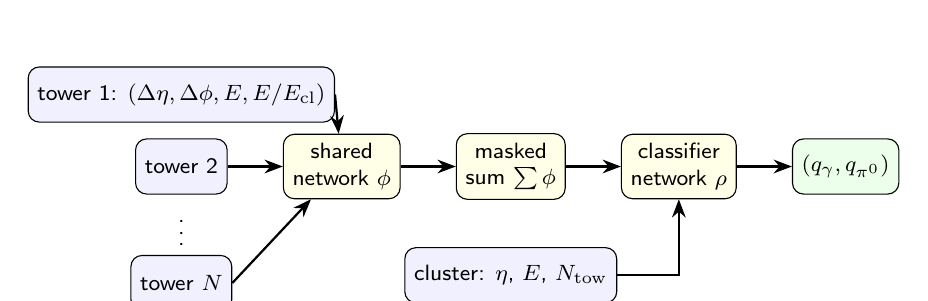
\begin{tikzpicture}[node distance=4mm and 7mm, every node/.style={font=\footnotesize},
 box/.style={draw, rounded corners, fill=blue!6, minimum height=7mm, align=center},
 arr/.style={-{Stealth}, thick}]
\node[box] (t1) {tower 1: $(\Delta\eta,\Delta\phi,E,E/E_{\rm cl})$};
\node[box, below=2mm of t1] (t2) {tower 2};
\node[below=0mm of t2] (dots) {$\vdots$};
\node[box, below=0mm of dots] (tn) {tower $N$};
\node[box, right=of t2, fill=yellow!10] (phi) {shared\\network $\phi$};
\node[box, right=of phi, fill=yellow!10] (sum) {masked\\sum $\sum\phi$};
\node[box, below=6mm of sum] (glob) {cluster: $\eta$, $E$, $N_{\rm tow}$};
\node[box, right=of sum, fill=yellow!10] (rho) {classifier\\network $\rho$};
\node[box, right=of rho, fill=green!8] (out) {$(q_\gamma,q_{\pi^0})$};
\draw[arr] (t1.east) -- (phi); \draw[arr] (t2.east) -- (phi); \draw[arr] (tn.east) -- (phi);
\draw[arr] (phi)--(sum); \draw[arr] (sum)--(rho); \draw[arr] (glob.east) -| (rho.south); \draw[arr] (rho)--(out);
\end{tikzpicture}\\[2pt]
{\small Figure 2 (schematic): a permutation-invariant tower-set classifier of the type described in [S31].}
\end{center}

\subsection{Training practice}
\begin{enumerate}
\item \textbf{Split} the labelled sample into training, validation (to choose hyperparameters and stop training) and test (used once,
for the final performance); 80/10/10 is common [S31].
\item \textbf{Balance and reweight.} If signal and background have different $p_T$ or $\eta$ spectra, the network can learn the spectrum
instead of the shower. Reweight one class so that both have the same kinematic distributions, or train in narrow bins.
\item \textbf{Scale features} to similar ranges; include only features that simulation models well.
\item \textbf{Watch overtraining}: compare score distributions on training and test samples; stop when validation loss stops falling.
\item \textbf{Fix the random seeds} and record the software versions so the model can be reproduced for review.
\end{enumerate}

\subsection{Measuring performance}
For a cut on the score, signal efficiency $\varepsilon_s$ and background efficiency $\varepsilon_b$ define one point; scanning the cut
traces the ROC curve. The area under it (AUC) equals the probability that a random signal scores higher than a random background. The
working point is chosen for the analysis, not for the AUC: for a yield measurement, maximise the expected significance
$S/\sqrt{S+B}$ or minimise the total uncertainty including the systematic on $\varepsilon_s$.

\conceptbox{Worked example (toy)}{Before ID, background exceeds signal by a factor 20 ($B/S=20$). A cut keeps $\varepsilon_s=0.90$ and
$\varepsilon_b=0.05$. Then $S/B=0.90/(20\times0.05)=0.9$: purity about 47\%. A tighter cut with $\varepsilon_s=0.70$,
$\varepsilon_b=0.02$ gives $S/B=1.75$ (purity 64\%) but loses 22\% of the signal. With $S_0=1000$ signal candidates before ID, the
significance $S/\sqrt{S+B}$ is $900/\sqrt{1900}=20.6$ versus $700/\sqrt{1100}=21.1$: almost equal. The choice is then decided by which
efficiency you can validate better in data.}

\subsection{From simulation to data}
A model trained on simulation sees simulated showers. Data differ (noise, calibration, shower-shape mis-modelling; [S17] needed to scale
the MC isolation energy to match data). The defence has four parts.
\begin{itemize}
\item \textbf{Control samples in data} with known labels: photons from conversions $\gamma\to e^+e^-$ and from well-separated
$\pi^0\to\gamma\gamma$ or $\eta\to\gamma\gamma$ pairs; pions from $K^0_S$; protons from $\Lambda$; electrons from conversions [S29, S31].
\item \textbf{Score comparisons}: the score distribution of a control sample in data and MC must agree; the ratio of cut efficiencies
is a scale factor with an uncertainty.
\item \textbf{Independent validation channels}: test on a process not used in training ($\phi\to K^+K^-$ in [S27]).
\item \textbf{Closure with injected effects}: distort the simulation in a known way and check that the method recovers it [S27].
\end{itemize}
Systematic uncertainties of an ML step are then assigned like any other cut (Module 9): vary the working point and apply the Barlow
test; use the data--MC efficiency difference in the control sample; retrain with a different generator or seed.

\subsection{Tools}
TMVA (inside ROOT) trains BDTs and MLPs and applies them in C++ through its reader, which fits a Fun4All module directly.
scikit-learn and XGBoost cover classical methods in Python; PyTorch covers networks. Models trained in Python can be exported (for
example to ONNX) for C++ inference; check which inference libraries the current \texttt{coresoftware} build provides before relying on
one. A minimal set-network classifier (toy, PyTorch) looks like this:
\begin{verbatim}
import torch, torch.nn as nn
class TowerSet(nn.Module):           # per-tower features: deta, dphi, E, E/Eclus
    def __init__(s, nf=4, nglob=3, h=64):
        super().__init__()
        s.phi = nn.Sequential(nn.Linear(nf,h), nn.ReLU(), nn.Linear(h,h), nn.ReLU())
        s.rho = nn.Sequential(nn.Linear(h+nglob,h), nn.ReLU(), nn.Linear(h,2))
    def forward(s, towers, mask, glob):  # towers [B,N,4], mask [B,N], glob [B,3]
        z = (s.phi(towers) * mask.unsqueeze(-1)).sum(1)   # masked sum pooling
        return s.rho(torch.cat([z, glob], 1))             # logits (gamma, pi0)
loss_fn = nn.CrossEntropyLoss()
\end{verbatim}

\connectbox{Two ML projects map onto your analysis. (1) A merged-$\pi^0$ selector at high $p_T$, trained on PYTHIA $\pi^0$ and single
photons with your EMCal smearing, validated on the $\pi^0$ peak region at $p_T$ where the photons are still resolved (pick events where
the classifier is applied to each photon of a resolved pair). (2) An EMCal energy-scale regression in $\eta$ and $\phi$ regions using the
$\pi^0$ mass as the likelihood target and the $\eta$ mass as the independent validation, the calorimeter analogue of [S27].}

%======================================================================
\section{Capstone project}
\hd{Goal} Write a two-page proposal for one improvement to your $\pi^0$/$\eta$ cross-section analysis that uses knowledge from outside
the EMCal, and present it to your advisor.

\subsection{Template}
Use these headings; each is a few sentences.
\begin{enumerate}
\item \textbf{Title and one-sentence aim.}
\item \textbf{Physics motivation}: which uncertainty or limitation of the current analysis it addresses; which factor of the master
formula (Module 9, Section 1) it changes.
\item \textbf{Current state}: how that factor is obtained now and its estimated uncertainty.
\item \textbf{Method}: data, triggers, simulation, reconstruction objects, and the algorithm.
\item \textbf{Validation}: closure test in simulation; a data control sample; a cross-check with an independent method.
\item \textbf{Expected gain}: a quantitative estimate (toy or simple calculation) of the improvement.
\item \textbf{Risks and fallbacks}: what could fail, and the reduced version that still delivers something.
\item \textbf{Timeline and deliverables}: milestones over 8--12 weeks; code, an analysis-note section, a TG presentation.
\end{enumerate}
A minimal LaTeX skeleton:
\begin{verbatim}
\documentclass[11pt]{article}\usepackage[margin=2cm]{geometry}
\begin{document}
\section*{Capstone: <title>}  \textbf{Aim.} ...
\paragraph{Motivation.} ...   \paragraph{Current state.} ...
\paragraph{Method.} ...       \paragraph{Validation.} ...
\paragraph{Expected gain.} ...\paragraph{Risks.} ...
\paragraph{Timeline.} weeks 1-2 ..., 3-6 ..., 7-10 ..., 11-12 write-up
\end{document}
\end{verbatim}

\subsection{Five worked project ideas}
\begin{enumerate}
\item \textbf{Track-based conversion veto and isolation.} Photons that convert before the EMCal produce $e^\pm$ tracks matched to the
cluster (track--calo matching, Module 8). Measure the conversion fraction in data versus simulation as a material check; use it to
correct the single-photon efficiency. Validation: conversion radius distribution matching known material.
\item \textbf{MBD trigger bias for $\pi^0$ events.} Measure $\varepsilon_{\rm MBD}$ for events with a high-$p_T$ $\pi^0$ using
photon-triggered data in which the MBD requirement was absent (or using ZDC- or clock-triggered samples), and compare with PYTHIA. Changes
a global factor of the cross section [S17 shows how large this factor can be for photons].
\item \textbf{Streaming-readout luminosity cross-check.} Count MBD coincidences in streaming data per bunch and compare with GL1
scalers; derive the pile-up correction from the bunch-by-bunch rate dependence (Module 9, Section 4.3).
\item \textbf{ML merged-$\pi^0$ selector} as in the box above, extending the $\pi^0$ spectrum to higher $p_T$; validation on resolved
pairs and on the $\eta$, which merges at much higher energy.
\item \textbf{Run-by-run EMCal scale from tower slopes and $\pi^0$ peaks.} Combine the tower-slope method (relative gains, as in [S42])
with the $\pi^0$ and $\eta$ peak positions (absolute scale) in run intervals; quantify the remaining scale uncertainty, which enters the
yield with power $m-1\approx6$. Builds directly on your Tower Slope MC studies.
\end{enumerate}

\subsection{Self-assessment before you present}
\begin{itemize}
\item Can you state which number in your error budget changes, and by roughly how much?
\item Is there a closure test, and is it non-trivial (independent samples)?
\item Is there a data-driven validation that does not use the same assumptions as the method?
\item Is the scope achievable in 8--12 weeks with a useful fallback?
\item Would a reviewer outside the Cold QCD or Jet TG understand the motivation from the first paragraph?
\end{itemize}

%======================================================================
\section{Optional hands-on exercises on SDCC}
These are suggestions; the text does not depend on them. Check paths and package availability in the current environment.
\begin{enumerate}
\item \textbf{Template practice.} Pick a public sPHENIX paper from the references and fill the six-question template in half a page.
\item \textbf{Tag-veto toy.} Generate $\pi^0\to\gamma\gamma$ decays with uniform $\alpha$; apply your EMCal smearing and a partner
threshold; plot the veto efficiency versus $\pi^0$ energy and compare with $1-2E_{\rm th}/E$.
\item \textbf{BDT versus cuts.} With TMVA, train a BDT on two or three shower moments of single photons and single $\pi^0$ from your
PYTHIA sample; compare the ROC with rectangular cuts; check overtraining.
\item \textbf{Set network.} Train the toy \texttt{TowerSet} model on tower lists from the same samples; balance the $p_T$
distributions first.
\item \textbf{Scale regression toy.} Inject a known $\phi$-dependent 2\% gain pattern into simulated towers, reconstruct $\pi^0$, and
recover the pattern by fitting peak positions in $\phi$ regions.
\end{enumerate}

%======================================================================
\section{Self-test questions}
Answers are in Appendix~\ref{app:answers}.
\begin{enumerate}
\item What do layer rotation [S25, S26], event mixing and like-sign pairs have in common?
\item Why does an over-efficient silicon seeding overcount particles, and what two handles reduce this?
\item The CME observable $\Delta\gamma$ has a background proportional to $v_2/N$. Explain qualitatively where it comes from.
\item Why is coherent $\rho^0$ photoproduction concentrated at very low $p_T$?
\item Why are photon-tagged jets at RHIC quark-enriched?
\item Write the expected $J/\psi$ yield formula and identify which factors also appear in your $\pi^0$ cross section.
\item Why do direct photons isolate initial-state spin effects?
\item For $E=8$~GeV and partner threshold 0.4~GeV, what fraction of $\pi^0$ escape a tag veto because the partner is too soft?
\item Show that minimising the expected cross-entropy gives $q^*(\mathbf x)=P(y=1\mid\mathbf x)$.
\item Why is a sum over towers used in the set network, rather than concatenating tower features?
\item Why did [S27] need both $K^0_S$ and $\Lambda/\bar\Lambda$, and why is $\phi\to K^+K^-$ a good validation?
\item In tag-and-probe, why must the probe be reconstructed without the layer under test?
\item Why does the tower-slope method exclude the low-energy part of the spectrum, and what does it not determine?
\item Name two control samples in data that provide pure photons and one that provides pure pions.
\end{enumerate}

%======================================================================
\section{Glossary}
\begin{description}[style=nextline,itemsep=0pt]
\item[AUC] Area under the ROC curve; probability that a random signal scores above a random background.
\item[CME] Chiral magnetic effect; charge separation along the magnetic field from a chirality imbalance.
\item[Cross-entropy] Negative log-likelihood loss for classification.
\item[Deep Sets] Permutation-invariant network $\rho(\sum\phi(x))$ over a set of inputs.
\item[Jet charge] $Q_k=\sum q_i(p_{T,i}/p_{T,\rm jet})^k$.
\item[LDME] Long-distance matrix element in NRQCD factorisation.
\item[QEC] Quarkonium energy correlator.
\item[ROC curve] Signal efficiency versus background efficiency (or rejection) as the score cut varies.
\item[Silicon seed] Track candidate from MVTX and INTT clusters, before TPC matching.
\item[Tag-and-probe] Efficiency measurement using objects selected without the element under test.
\item[Tag veto] Rejection of photon candidates that form a $\pi^0$ or $\eta$ mass with another cluster.
\item[Tower-slope calibration] Relative gain calibration by matching each tower's spectrum to its symmetric neighbours.
\item[Tracklet] Pair of hits in two silicon layers pointing to the vertex.
\item[UPC] Ultra-peripheral collision; photon-induced interaction at large impact parameter.
\end{description}

%======================================================================
\section{References}
\begin{enumerate}[label={[\arabic*]},itemsep=0pt]
\item sPHENIX Collab., Measurement of charged hadron multiplicity in Au+Au at 200 GeV, arXiv:2504.02240, JHEP 08 (2025) 075.
\item sPHENIX Collab., Measurement of the transverse energy density in Au+Au at 200 GeV, arXiv:2504.02242, PRC 112 (2025) 024908.
\item sPHENIX Collab., Dijet transverse momentum imbalance and acoplanarity in $p$+$p$ at 200 GeV,\\ arXiv:2606.17184.
\item sPHENIX Collab., Isolated prompt photon production in $p$+$p$ at 200 GeV, arXiv:2607.03892.
\item The ladder and readout cables of the Intermediate Silicon Strip Detector for sPHENIX, arXiv:2503.09105.
\item sPHENIX INTT test beam, NIM-A 1086 (2026) 171312, arXiv:2509.00908.
\item Aidala et al., Design and beam test results for the sPHENIX EMCal and HCal prototypes, IEEE Trans.\ Nucl.\ Sci.\ (2018)
2901--2919, arXiv:1704.01461.
\item PHENIX Collab., An Upgrade Proposal from the PHENIX Collaboration, arXiv:1501.06197.
\item sPHENIX Public Results page, \url{https://www.sphenix.bnl.gov/PublicResults}.
\end{enumerate}
\textbf{School talks} (sPHENIX School 2026, BNL, July 2026):
{[S04]} G.\ Nukazuka, M.\ Sarsour, `Cold QCD TG Analysis Opportunities';
{[S05]} M.\ Mitrankova, R.\ Belmont, `Bulk TG Analysis Opportunities';
{[S17]} Y.\ Go, `Photon Reconstruction';
{[S25]} H.-R.\ Jheng, `Charged hadron multiplicity in O+O using silicon seeds';
{[S26]} C.-W.\ Shih, `Charged-hadron multiplicity in O+O collisions';
{[S27]} A.\ Patton, `Machine Learning Momentum Scale Correction';
{[S28]} T.\ Kikuchi, `INTT hit detection efficiency study';
{[S29]} B.\ Sayki, `J/psi energy correlators in $p$+$p$';
{[S30]} J.\ Hwang, `Transverse single-spin asymmetries of isolated prompt photons';
{[S31]} R.\ Koike, `Neural network discrimination of isolated photons';
{[S32]} S.-Y.\ Chen, `What I have done and what I plan to do next';
{[S34]} I.\ Omae, `Measurement of $v_2$ in Au+Au';
{[S35]} R.\ Takaaze, `First Step in Jet Analysis';
{[S37]} J.\ Singh, `Constraining the CME using SDM';
{[S38]} K.\ Gable, `Angular correlations of $\phi$ mesons and high-$p_T$ hadrons';
{[S39]} L.\ Mwibanda, `UPC $\rho^0$ production in O+O and Au+Au, simulation';
{[S40]} M.\ I.\ Abdulhamid, `Joint jet mass and charge for quark/gluon jet separation';
{[S41]} T.\ Harada, `Vernier Scan analysis of $p$+$p$ and O+O in Run 25';
{[S42]} A.\ M.\ Khan, `HCal Calibration studies';
{[S43]} J.\ Park, `Jet Analysis'.

%======================================================================
\appendix
\section{Answers}\label{app:answers}
\begin{enumerate}
\item Each destroys the physical correlation between the two objects of a pair while keeping the detector acceptance and single-object
distributions, so the result estimates combinatorial background.
\item Seeding keeps many candidates per particle (combinatorial and duplicate seeds) to maximise efficiency, expecting TPC matching to
remove fakes. Handles: a vertex-association cut on the seed's closest approach to the vertex, and pruning seeds that share clusters.
\item Local charge conservation produces opposite-sign pairs close in azimuth; flow aligns these pairs preferentially with the reaction
plane, which gives a positive opposite-minus-same-sign correlation proportional to $v_2$ and diluted by multiplicity $N$.
\item In coherent production the photon scatters off the whole nucleus, which stays intact; the momentum transfer is limited by the
nuclear form factor to about $\hbar c/R_A$, of order 0.1~GeV.
\item Direct photons are produced mostly by $qg\to q\gamma$, which leaves a quark recoiling against the photon.
\item $N=N_{\rm MB}(\sigma_{J/\psi}/\sigma_{\rm MBD})\varepsilon_{\rm MBD}B_{ee}A\,\varepsilon_{\rm trig}\varepsilon_{\rm reco}$.
Shared with your analysis: $N_{\rm MB}/\sigma_{\rm MBD}$ (luminosity), $\varepsilon_{\rm MBD}$ for signal events, branching ratio,
acceptance, trigger turn-on and reconstruction efficiency.
\item Photons do not fragment and do not interact strongly after production, so there are no final-state (Collins-type) effects.
\item Probability $=2E_{\rm th}/E=0.8/8=10\%$.
\item At fixed $\mathbf x$ the expected loss is $-[\pi\ln q+(1-\pi)\ln(1-q)]$. Its derivative is $-\pi/q+(1-\pi)/(1-q)=0$, so $q=\pi$.
\item A sum is permutation invariant and works for any number of towers; concatenation would depend on an arbitrary tower order and a
fixed length.
\item $K^0_S$ fixes the charge-symmetric scale $\epsilon$; $\Lambda$ and $\bar\Lambda$ have the heavy and light daughters with opposite
charges, which separates the charge-odd term $\delta$. $\phi\to K^+K^-$ was not used in training (neither the decay nor kaons), so it
is an independent test.
\item Otherwise the probe would be biased toward events where the tested layer has a hit, and the efficiency would be overestimated.
\item Noise, pedestal shifts, zero suppression and trigger thresholds distort the low-energy region and are not gain effects. The
method gives relative gains within a ring, not the absolute energy scale.
\item Photons: conversions $\gamma\to e^+e^-$ (via the pair) and well-separated photon pairs from $\pi^0$ or $\eta$ in the mass
window. Pions: $K^0_S\to\pi^+\pi^-$.
\end{enumerate}
\end{document}
